% !TeX spellcheck = es_ES
\documentclass[12pt, titlepage]{article}
\usepackage[utf8]{inputenc}
\usepackage[spanish]{babel}
\usepackage{float}
\usepackage[letterpaper, margin=2.5cm]{geometry}
\usepackage[nottoc,notlot,notlof]{tocbibind} % Hace que se agregen las referencias al indice
\usepackage{url}
\usepackage{graphicx} 
\usepackage{listings}
\usepackage{color}
\definecolor{dkgreen}{rgb}{0,0.6,0}
\definecolor{gray}{rgb}{0.5,0.5,0.5}
\definecolor{mauve}{RGB}{253,151,31}

\lstset{frame=tb,
	language=Sql,
	aboveskip=3mm,
	belowskip=3mm,
	showstringspaces=false,
	columns=flexible,
	basicstyle={\small\ttfamily},
	numbers=none,
	numberstyle=\tiny\color{gray},
	keywordstyle=\color{blue},
	commentstyle=\color{dkgreen},
	stringstyle=\color{mauve},
	breaklines=true,
	breakatwhitespace=true,
	tabsize=2,
	morekeywords={use}
}

\title{Reporte: Práctica 9}
\author{Carlos Tonatihu Barrera Pérez \\ Profesor: Hernández Contreras Euler \\ Bases de Datos \\ Grupo: 2CM1 }

\begin{document}
	\maketitle
	\tableofcontents
	\section{Marco Teórico}
	Esperando que este con madre
	\section{Desarrollo}
	En esta practica se trabajan transacciones sobre la tabla tienda de la base de datos elektra, la cual ya tiene datos, las operaciones que se realizaran sobre esta tabla son similares a las que se trabajaron con la tabla cliente en el salón de clases.
	
	Comenzamos con la siguiente transacción.
	
	\begin{lstlisting}
	begin;
	select * from tienda where idTienda between 90 and 777;
	insert into tienda(idTienda, nombre, estado, tel) values(777, "MEGA ELEKTRA", "Chiapas", "7777777777");
	select * from tienda where nombre like "mega%" and tel like "777%";
	rollback;
	select * from tienda where nombre like "mega%" and tel like "777%";
	\end{lstlisting}
	
	En la imagen \ref{fig:uno} podemos observar que al hacer el rollback dentro del modo transacción el registro que se había dado de alta desaparece y es como si no se hubiese hecho, el resto de operaciones realizadas son igual que en otras practicas.
	
	\begin{figure}[H]
		\begin{center}
			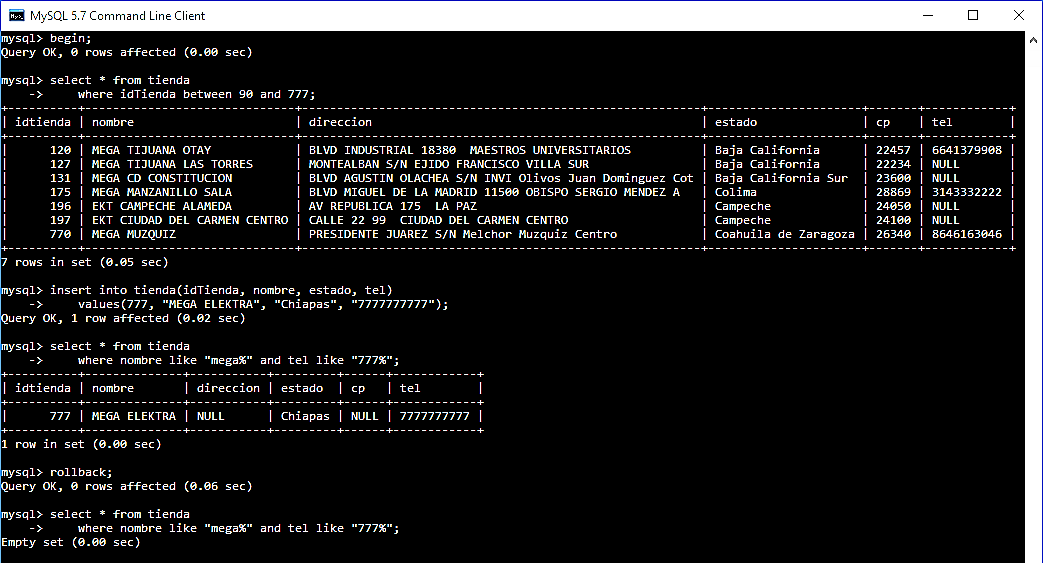
\includegraphics[width=\textwidth]{img/1.png}		
			\caption{Transacción con rollback}
			\label{fig:uno}
		\end{center}
	\end{figure}
	
	Continuamos con la siguiente transacción.
	\begin{lstlisting}
	begin;
	select count(*) from tienda;
	select * from tienda where nombre like "mega%" and tel like "777%";
	insert into tienda(idTienda, nombre, estado, tel) values(777, "MEGA ELEKTRA", "Chiapas", "7777777777");
	select * from tienda where nombre like "mega%" and tel like "777%";
	\end{lstlisting}
	
	En esta no se realiza un rollback pero al cerrar la consola la operación de escritura no se realizara por lo que es como si nada hubiese pasado.
	
	\begin{figure}[H]
		\begin{center}
			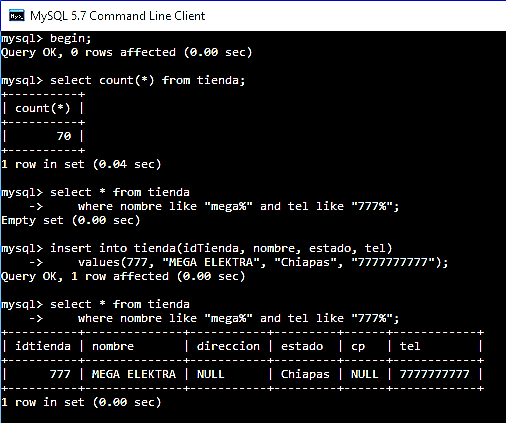
\includegraphics[width=\textwidth]{img/dos.png}
			\caption{Transacción que no surtira efecto}
			\label{fig:dos}
		\end{center}
	\end{figure}
	
	La tercera transacción es la siguiente en donde realizamos un commit.
	
	\begin{lstlisting}
	begin;
	select count(*) from tienda;
	insert into tienda(idTienda, nombre, estado, tel) values(777, "MEGA ELEKTRA", "Chiapas", "7777777777");
	select * from tienda where nombre like "mega%" and tel like "777%";
	commit;
	select * from tienda where nombre like "mega%" and tel like "777%";
	\end{lstlisting}
	
	Al hacer un commit la operación de escritura se llevara a cabo y permanecerá incluso después de cerrar la consola.

	\begin{figure}[H]
		\begin{center}
			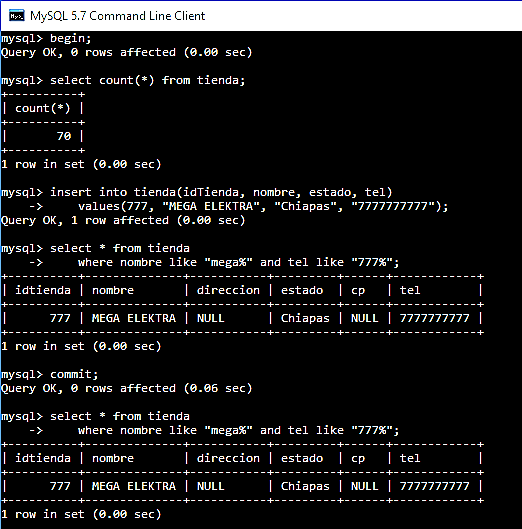
\includegraphics[width=\textwidth]{img/tres.png}
			\caption{Transacción con commit}
			\label{fig:tres}
		\end{center}
	\end{figure}
	
	En esta transacción también realizamos un commit.
	\begin{lstlisting}
	begin;
	select count(*) from tienda;
	insert into tienda(idTienda, nombre, estado, tel) values(778, "OTRO ELEKTRA", "Campeche", "6666666666");
	select * from tienda where nombre like "otro%" and tel like "666%";
	commit;
	\end{lstlisting}
	
	\begin{figure}[H]
		\begin{center}
			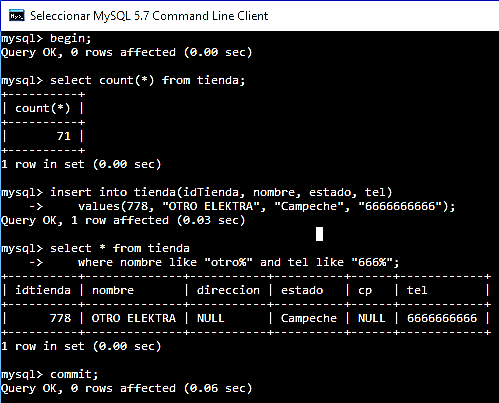
\includegraphics[width=\textwidth]{img/cuatro.png}
			\caption{Transacción con commit}
			\label{fig:cuatro}
		\end{center}
	\end{figure}

	Y cerramos la terminal y comprobamos los cambios como se muestra en la figura \ref{fig:cinco}.
	
	\begin{figure}[H]
		\begin{center}
			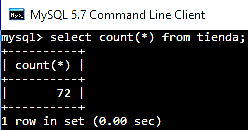
\includegraphics[width=8cm]{img/cinco.png}
			\caption{Cambios efectuados después de cerrar la consola gracias a la instrucción commit}
			\label{fig:cinco}
		\end{center}
	\end{figure}
	
	
	En esta parte se trabaja con más de una consola las cuales se pueden diferenciar gracias a su color de fondo.
	En la terminal negra iniciamos el modo de transacciones y ejecutamos la siguiente consulta.
	
	\begin{figure}[H]
		\begin{center}
			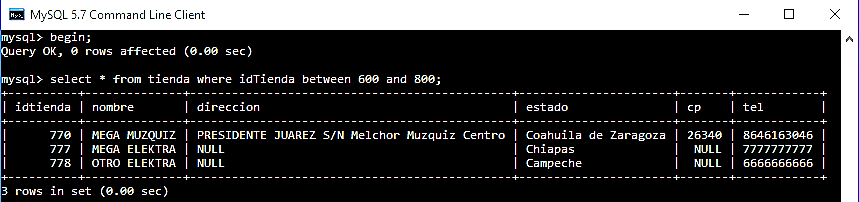
\includegraphics[width=\textwidth]{img/seis.png}
			\caption{Resultados de la consulta}
			\label{fig:seis}
		\end{center}
	\end{figure}

	En la consola blanca hacemos lo mismo pero sin iniciar una nueva transacción, por lo que sera una simple consulta. Y podremos apreciar que para este punto no hay diferencia.
	
	\begin{figure}[H]
		\begin{center}
			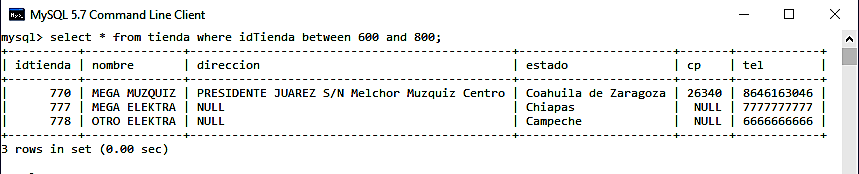
\includegraphics[width=\textwidth]{img/siete.png}
			\caption{Resultados de la consulta igual a los de la imagen anterior}
			\label{fig:siete}
		\end{center}
	\end{figure}

	En la consola negra damos de alta una nueva tienda y realizamos una consulta.
	
	\begin{figure}[H]
		\begin{center}
			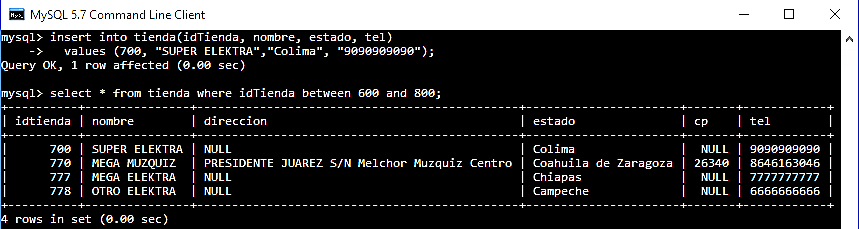
\includegraphics[width=\textwidth]{img/ocho.png}
			\caption{Alta realizada correctamente.}
			\label{fig:ocho}
		\end{center}
	\end{figure}

	En la consola blanca realizamos la misma consulta pero se podrá apreciar que los cambios parecen no haber surtido efecto.
	
	\begin{figure}[H]
		\begin{center}
			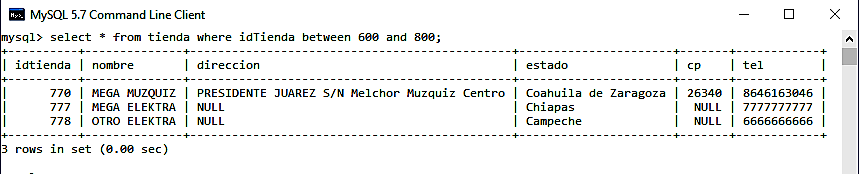
\includegraphics[width=\textwidth]{img/nueve.png}
			\caption{La consulta es diferente a la anterior.}
			\label{fig:nueve}
		\end{center}
	\end{figure}

	Esto se debe a que no hemos realizado el commit correspondiente en la terminal negra por lo que procedemos a realizarlo y volver a realizar la consulta en la consola blanca.
	
	\begin{figure}[H]
		\begin{center}
			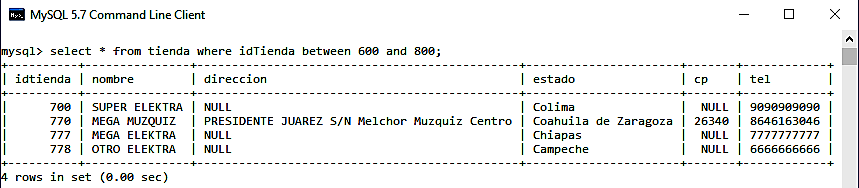
\includegraphics[width=\textwidth]{img/diez.png}
			\caption{Esta vez si se pueden observar los cambios que se realizaron.}
			\label{fig:diez}
		\end{center}
	\end{figure}

	Ahora veremos otra característica del uso de transacciones el cual es el poder hacer bloqueos de escritura y lectura sobre tablas, el funcionamiento de dichos bloqueos se puede observar en los siguientes ejercicios.
	
	Realizamos un bloque de lectura sobre la tabla tienda en la consola negra y realizamos una consulta.
	
	\begin{figure}[H]
		\begin{center}
			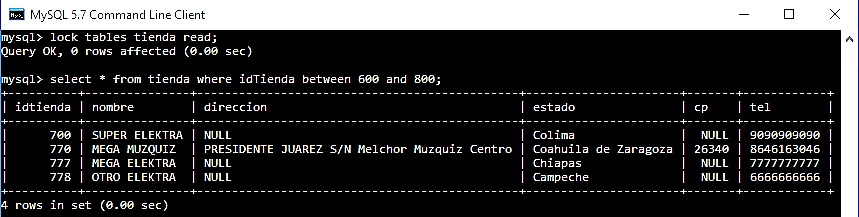
\includegraphics[width=\textwidth]{img/once.png}
			\caption{Consulta sobre la tabla bloqueada.}
			\label{fig:once}
		\end{center}
	\end{figure}
	
	En este caso la única tabla que podrá ser consultada en la consola negra es tienda y solo se podrán hacer operaciones de lectura.
	
	Por otro lado, en la terminal verde se podrá realizar cualquier acción sobre las tablas de la base de dados a excepción de la tabla tienda en la cual solo se podrán hacer bloqueos de lectura debido a que este bloqueo es compartido.
	
	\begin{figure}[H]
		\begin{center}
			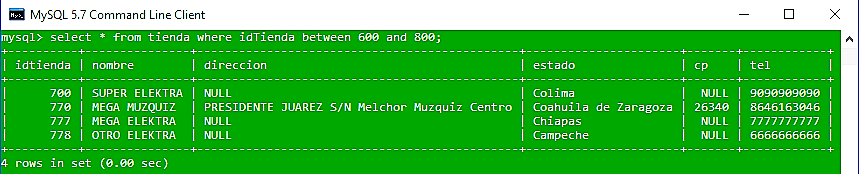
\includegraphics[width=\textwidth]{img/doce.png}
			\caption{Consulta sobre la tabla bloqueada en la terminal verde.}
			\label{fig:doce}
		\end{center}
	\end{figure}
	
	La ultima transacción es la siguiente. En donde se comienza por desbloquear todas las tablas y bloquear la tabla tienda en modo escritura, realizar una alta y una consulta.
	
	\begin{figure}[H]
		\begin{center}
			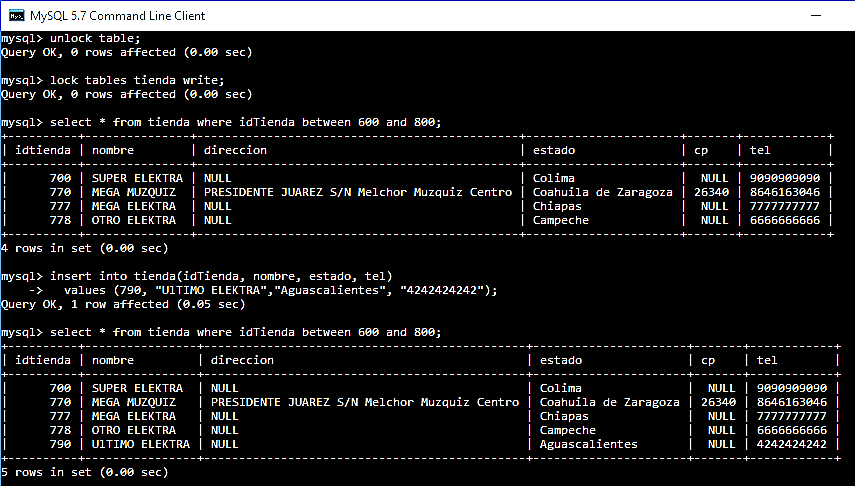
\includegraphics[width=\textwidth]{img/trece.png}
			\caption{Operaciones de lectura y escritura sobre una tabla bloqueada.}
			\label{fig:trece}
		\end{center}
	\end{figure}

	Al igual que con en bloqueo de lectura en este caso solo se podrá trabajar con la tabla tienda en la terminal negra y se podrán realizar operaciones de lectura y escritura.
	
	\begin{figure}[H]
		\begin{center}
			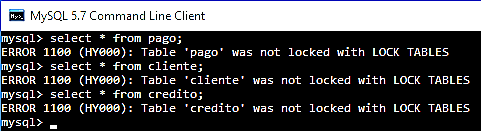
\includegraphics[width=\textwidth]{img/catorce.png}
			\caption{Solo podemos acceder a la tabla tienda en la terminal negra.}
			\label{fig:catorce}
		\end{center}
	\end{figure}
	
	Mientras tanto en la consola verde podemos observar que ocurre lo siguiente. La consulta a la tabla tienda no se realiza, sin embargo, si desbloqueamos la tabla tienda en la consola negra la consulta se llevara a cabo.
	
	\begin{figure}[H]
		\begin{center}
			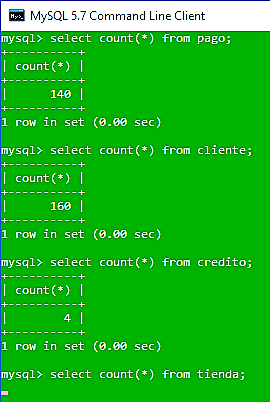
\includegraphics[width=8cm]{img/quince.png}
			\caption{En la otra terminal podemos acceder a todas las tablas a excepción de la tabla tienda que esta bloqueda en la otra consola.}
			\label{fig:quince}
		\end{center}
	\end{figure}
	
	\section{Conclusiones}
	El uso de transacciones y bloqueos nos permiten brindarle a nuestra base de datos una nueva herramienta para poder conservar la integridad de los datos y con eso evitar errores de escritura y consulta que pueden darse si es que ocurre un error de conexión a la base de datos o de cualquier otra índole que impida la ejecución de alguna operación. Así, solo se llevaran a cabo modificaciones en la base de datos si todas las operaciones que se tienen que realizar se ejecutan correctamente y en caso contrario se lograra deshacer todos los cambios que se realizaron para así evitar incoherencias en nuestros datos.
	\bibliography{bibliografia} 
	\bibliographystyle{ieeetr}
\end{document}